\PassOptionsToPackage{quiet}{fontspec} % suppress the warnings

\documentclass[zihao = -4, linespread = 1.5]{ctexart}

\usepackage{nag} % 检测宏包是否过期











%%%%%%%%%%%%%%%%%%
% 标题格式
%%%%%%%%%%%%%%%%%%
\ctexset{
    contentsname = {目\quad 录},
    %appendix/name = {附\quad 录}, % NK似乎没打算让我们有多个附录
    proofname = {\indent \normalfont \heiti 证},
    bibname = {参考文献},
    %
    section/name = {,、},
    section/number = \chinese{section},
    section/aftername = \hspace{0pt},
    section/format += \zihao{-3},
    %
    subsection/name =  {(,)},
    subsection/number = \chinese{subsection},
    subsection/aftername = \hspace{0pt},
    subsection/format += \zihao{4},
    %
    subsubsection/number = \arabic{subsubsection},
    subsubsection/name = {,.},
    %subsubsection/aftername = \hspace{0pt},
    subsubsection/format += \zihao{-4}
}

\pagestyle{plain} % 取消页眉




%%%%%%%%%%%%%%%%%%
% 数学公式、定理环境
%%%%%%%%%%%%%%%%%%
\usepackage{amsmath, amsfonts, amsthm}
\usepackage{amssymb, latexsym}
\usepackage{bm} % 数学字体
\usepackage{bbm}

%\newtheorem*{proof}{\hspace{2em}证明} % ams宏包自带proof
\theoremstyle{plain}
\newtheorem{theorem}{定理}
\newtheorem{corollary}{推论}
\newtheorem*{lemma}{引理}
\newtheorem{proposition}{命题}
\newtheorem{assumption}{假设}

\theoremstyle{definition}
\newtheorem{definition}{定义}
\newtheorem{example}{例}

\theoremstyle{remark}
\newtheorem{remark}{\indent \normalfont \heiti 注}

\renewcommand\qedsymbol{\ensuremath{\blacksquare}}
%\numberwithin{equation}{section} % 公式根据 section 编号
%\renewcommand{\proofname}{\indent \normalfont \heiti 证} % 已经在ctex中设置了





%%%%%%%%%%%%%%%%%%
% 图表
%%%%%%%%%%%%%%%%%%
\usepackage[inline]{enumitem} % 可以自定义列表编号,提供行内列表
\usepackage[labelsep=quad]{caption} % 设置表格标题间距 用space太窄 quad太宽 MD
\captionsetup[table]{skip=10pt}
%\captionsetup[lstlisting]{name=代码}
\usepackage{subcaption}
\usepackage{booktabs} % 三线表
\usepackage{diagbox} % 对表头用斜线分割
\usepackage{multirow} % 纵向合并单元格
%\usepackage{tabu} % 该包已经停止维护
%\usepackage{tabularx} % 为与hyperref兼容,在200行导入
\usepackage{longtable} % 跨页表格
\usepackage{multirow} % 表格跨行单元格
\usepackage{graphicx} % 插入图片
\usepackage{float}




%%%%%%%%%%%%%%%%%%
% 目录
%%%%%%%%%%%%%%%%%%
\usepackage[nottoc,numbib]{tocbibind} % 参考文献出现在目录中
\usepackage[subfigure, titles]{tocloft} % 目录 加点 但会改变 “目录”二字 % 根据文档,这两个option都要加
\renewcommand{\cftsecleader}{\cftdotfill{\cftdotsep}}
\setlength\cftsubsubsecnumwidth{1.5em} % 修复目录中subsubsection过深的bug % 调整了package顺序后,bug消失了……




%%%%%%%%%%%%%%%%%%
% 脚注
%%%%%%%%%%%%%%%%%%
\usepackage{pifont}  % footnote格式
\renewcommand\thefootnote{\ding{\numexpr171+\value{footnote}}}
\usepackage[perpage]{footmisc} % 脚注每页从1开始编号
%\renewcommand{\footnotesize}{\zihao{-5}} % 默认就是小五


%%%%%%%%%%%%%%%%%%
% 字体
%%%%%%%%%%%%%%%%%%
\usepackage[T1]{fontenc}  % 使用Times New Roman 字体
\usepackage{mathptmx}% https://liam.page/2017/01/10/Times-New-Roman-and-LaTeX/
%\usepackage{newtxtext, newtxmath} % 另一种方法



%%%%%%%%%%%%%%%%%%
% 其它
%%%%%%%%%%%%%%%%%%
\usepackage{siunitx} % 单位、数字
\usepackage{pdfpages} % 插入PDF文件, 用于插入封面
%\usepackage{soul} % 广义文本装饰,但删除线无法用于中文
%\usepackage[normalem]{ulem} % 删除线,在中文会出现重心下移
\usepackage{xeCJKfntef} % 支持中文的删除线
\usepackage{wasysym} % emoji
\usepackage{xurl} % 允许超链接随时换行
%\usepackage[htt]{hyphenat} % 允许 texttt 换行。 wdnmd 会导致二十几个warning
%\usepackage[utf8]{inputenc} % inputenc is abandoned because it does absolutely nothing with XeTeX or LuaLaTeX.
%\usepackage[english]{babel} % 与CTEX冲突



%%%%%%%%%%%%%%%%%%
% 代码、伪代码
%%%%%%%%%%%%%%%%%%
\usepackage{algorithm} % 伪代码
\usepackage{algorithmic} % 伪代码
\usepackage{listings} % 代码
\renewcommand{\lstlistingname}{代码}%  但这又会导致cleveref失效,
\renewcommand{\lstlistlistingname}{代码目录}%
\floatname{algorithm}{算法}
\renewcommand{\algorithmicrequire}{\heiti{输入:}}
\renewcommand{\algorithmicensure}{\heiti{输出:}}


\usepackage{xcolor}  % 定义颜色
\definecolor{codegreen}{rgb}{0,0.5,0} % rgb(0, 128, 0) % 3个颜色用于代码
\definecolor{codegray}{rgb}{0.5,0.5,0.5}
\definecolor{codepurple}{rgb}{0.64,0.08,0.08} % rgb(163, 21, 21)

\definecolor{nankaipurple}{rgb}{0.49,0.05,0.43} % 南开紫 rgb(126, 12, 110)  % 2个颜色用于超链接
%\definecolor{darkred}{rgb}{0.5, 0, 0}
\definecolor{darkgreen}{rgb}{0, 0.6, 0}
\definecolor{linkblue}{rgb}{0.01, 0.40, 0.84} % rgb(3, 102, 214) github textlint

\lstdefinestyle{mystyle}{
    commentstyle=\color{codegreen},
    keywordstyle=\color{blue},
    numberstyle=\tiny\color{codegray},
    stringstyle=\color{codepurple},
    basicstyle=\ttfamily\small,
    breakatwhitespace=false,
    breaklines=true,
    captionpos=b,
    keepspaces=true,
    numbers=left,
    numbersep=5pt,
    showspaces=false,
    showstringspaces=false,
    showtabs=false,
    tabsize=2
}

\lstset{style=mystyle}






%%%%%%%%%%%%%%%%%%
% 必须在最后导入的东西
%%%%%%%%%%%%%%%%%%
\usepackage[linkcolor=nankaipurple,citecolor=darkgreen,urlcolor=linkblue, CJKbookmarks, colorlinks]{hyperref} % 超链接。应最后导入
%\usepackage[linkcolor=blue,citecolor=blue,CJKbookmarks]{hyperref} % 若不希望高亮超链接,使用这一行而非上一行
\hypersetup{linktoc = page} % 目录只高亮页码

\usepackage{tabularx} % 有个示例用了。 % 需要在hyperref后引用
\usepackage[a4paper, left=2.8cm,right=2.8cm,top=2.54cm,bottom=2.54cm]{geometry} % 页边距 例外:在hyperref后导入





% 若希望没有冲突,将以下所有命令注释
% 你将无法使用它的\cref命令,可以用\ref替代
%  \usepackage[nameinlink]{cleveref}
%  \crefformat{section}{#2第#1节#3}      % #2 #3 所包围的是作为链接的范围。 若是“第#2#1#3节” 则只有数字作为超链接的一部分
%  \crefformat{subsection}{#2第#1小节#3}
%  \crefformat{subsubsection}{#2第#1小小节#3}
%  \crefformat{paragraph}{#2第#1段#3}
%  \crefformat{subparagraph}{#2第#1小段#3} %
%  \crefformat{equation}{#2式~(#1)#3}
%  \crefformat{figure}{#2图~#1#3}
%  \crefformat{table}{#2表~#1#3}
%  \crefformat{theorem}{#2定理~#1#3}
%  \crefformat{corollary}{#2推论~#1#3}
%  %\crefformat{lemma}{#2引理~#1#3} % 没法引用引理
%  \crefformat{proposition}{#2命题~#1#3}
%  \crefformat{assumption}{#2假设~#1#3}
%  \crefformat{definition}{#2定义~#1#3}
%  \crefformat{example}{#2例~#1#3}
%  \crefformat{remark}{#2注~#1#3}
%  \crefformat{algorithm}{#2算法~#1#3}
%  \crefformat{listing}{#2代码~#1#3}




%%%%%%%%%%%%%%%%%%
% 自定义 命令和环境
%%%%%%%%%%%%%%%%%%

\newcommand{\NKUInputCover}{  % 插入封面
    \pagenumbering{gobble} % 取消页码
    
\includepdf[pages=1,pagecommand={},width=\textwidth,trim=28mm 25.4mm 28mm 25.4mm, clip]{cover/cover1.pdf} % 左 下 右 上
    
\includepdf[pages=1,pagecommand={},width=\textwidth,trim=28mm 25.4mm 28mm 25.4mm, clip]{cover/cover2.pdf}
    \pagenumbering{arabic}
}


\newenvironment{NKUAbstractZh} % 中文摘要
{
    \renewcommand{\abstractname}{\zihao{4} 摘\quad 要}
    \pagenumbering{Roman}
    \begin{abstract}\zihao{-4}
}
{
    \end{abstract}
    \newpage
}

\newenvironment{NKUAbstractEn} % 英文摘要
{
    \renewcommand{\abstractname}{\zihao{4} Abstract}
    \begin{abstract}\zihao{-4}
}
{
    \end{abstract}
    \newpage
}

\newcommand{\NKUAppendixSection}{ % 附录节
    \clearpage
    % 写法一:默认的 \appendix 命令
    %\appendix % 该行以后的章节都无编号
    %\ctexset{section/aftername = \hspace{6pt}} % 恢复间距
    %
    % 写法二:由于NK应该是只需要一个目录,因此采用了下面的方法
    \setcounter{secnumdepth}{0} % 抑制section的编号
    \section{\texorpdfstring{附\quad 录}{附录}} % 正常情况下应该是\section{附\quad 录},但为了兼容PDF书签功能这么写
}


\newcommand{\NKUThanksSection}{ % 致谢节
   \clearpage
    \section{\texorpdfstring{致\quad 谢}{致谢}} % 正常情况下应该是\section{致\quad 谢},但为了兼容PDF书签功能这么写
}


\begin{document}
\NKUInputCover % 插入封面 cover1.pdf 和 cover2.pdf


\begin{NKUAbstractZh}
此模板根据\href{http://jwc.nankai.edu.cn/bylwwsjw/list.htm}{《南开大学本科毕业论文(设计)指导手册2018 》}(以下简称《指导手册》)的要求制作,这是目前最新的要求。
由于作者专业的原因,本模板花较大篇幅展示了如何排版数学公式、定理和证明。希望此模板能帮助更多正在写论文的同学。

{\heiti 下载方式:}
\begin{itemize}
  \item 你可以在 GitHub: \href{https://github.com/skyline77/NKU-biyelunwen-2021}{\texttt{NKU-biyelunwen-2021}} 下载文件,在本地使用。
            若无法登录GitHub,也可以在\href{https://pan.baidu.com/s/1RnDI7RqW5qRcyaw8ZpYMTw}{百度网盘}下载,提取码:\texttt{p4qv}。
  \item 使用 Overleaf 的模板:\href{https://www.overleaf.com/latex/templates/nku-bi-ye-lun-wen-2021/svxybkzxyycp}{NKU-毕业论文-2021} 在线编程。
\end{itemize}

{\heiti 使用建议:}
\begin{itemize}
  \item 请使用 XeLaTeX 进行编译\footnote{在Overleaf上切换编译器的方式见\href{https://www.overleaf.com/learn/how-to/Changing_compiler}{文章}。}。
  \item 使用模板时,建议不要删除原来的内容,将其注释即可,以备日后需要。
  \item 若不希望将超链接上色,将\texttt{preamble.tex}中导入\texttt{hyperref}的colorlinks选项去掉(位于文件约 190 行)。
  \item 你需要自行在\texttt{cover1.docx}中制作封面并导出为\texttt{cover1.pdf},以替换作者的封面。\CJKunderline{不要使用作者的封面\blacksmiley{}}
  \item 推荐在 \href{https://www.tablesgenerator.com/}{Tables Generator} 网站制作表格,使用 \href{https://mathpix.com/ocr/}{Mathpix}\footnote{该软件经由阿里系某二手交易软件赋能后可发挥最大功效。} 软件书写数学公式,它们能很大地提升写作效率。
\end{itemize}

最后,由于本人水平有限,模板仍存在不足,欢迎指出,本人将会\CJKsout{量力而为}尽力完善。联系方式:
\begin{enumerate*}[label=(\arabic*)]
   \item 微信:\texttt{zp18102190105};
  \item QQ:\texttt{602795339};
  \item 邮箱:\texttt{602795339@qq.com}。
\end{enumerate*}
\par\noindent\textbf{关键词:}南开大学毕业论文;\LaTeX;数学公式;定理环境;代码
\end{NKUAbstractZh}



\begin{NKUAbstractEn}
If you skip the previous abstract in Chinese and come here for help, this template is not for you\smiley{}.
\par\noindent\textbf{Keywords: }\LaTeX{} template; impatient author
\end{NKUAbstractEn}



\tableofcontents % 生成目录。注意要连续两次编译才能正确生成目录
\newpage
\pagenumbering{arabic} % 改用阿拉伯数字页码



\section{基础}\label{sec:fundamental}
\subsection{节、小节、小小节、段落}
\subsubsection{这是小小节1.1.1}
此处是1.1.1小小节。
完整的层次结构为:section(节)---subsection(小节)---subsubsection(小小节)---paragraph(段)---subparagraph(小段)。为清晰起见,不建议使用过多层次。作者的毕业论文中只使用了前3层。
\subsection{列表}
无序列表:
\begin{itemize}
  \item 中文
  \item English
\end{itemize}

有序列表:
\begin{enumerate}
  \item 中文
  \item English
\end{enumerate}

有序列表有行内的版本:\begin{enumerate*}[label=(\arabic*)]
\item 中文;
\item English。
\end{enumerate*}


列表可以相互嵌套使用(至多四层):
\begin{enumerate}
  \item 中文
  \begin{enumerate}
    \item 古代汉语
    \item 现代汉语
    \begin{enumerate}
      \item 口语
      \begin{itemize}
        \item 普通话
        \item 方言
      \end{itemize}
      \item 书面语
    \end{enumerate}
  \end{enumerate}
  \item English
  \item 日本語
\end{enumerate}

\subsection{脚注、文献引用和交叉引用}\label{subsec:crossRef}
使用 \texttt{\textbackslash footnote}输入脚注\footnote{这是脚注。 }。使用 \texttt{\textbackslash cite}引用文献,如 \cite{PangQingShan}、\cite{HuGang, LiMing, Dupont}、\cite{url}(引用之前需要在\nameref{sec:bib}中定义)。

交叉引用,即我们使用 \texttt{\textbackslash label}命令在某处标记,以后再用 \texttt{\textbackslash ref}命令引用该标记。
使用交叉引用功能的好处是, \texttt{\textbackslash ref}命令引用的内容会随着 \texttt{\textbackslash label}命令所在的位置、环境
自动变化。
示例:此处是第\ref{sec:fundamental}节的第\ref{subsec:crossRef}小节,小节的标题是“\nameref{subsec:crossRef}”,
位于文档的第~\pageref{subsec:crossRef} 页。% ~ 是不换行空格,防止“第”字出现在行末,“2页”出现在下一行。

%你也可以使用 \texttt{cleveref}包的 \texttt{\textbackslash cref}功能,本模板对该命令进行了汉化。
%示例:此处是\cref{sec:fundamental}的\cref{subsec:crossRef},在下文中你可以看到\cref{fig:scatter}、
%\cref{eq:1}、\cref{def:supremum}、\cref{thm:monotone}、\cref{algo:1}和\cref{code:fibonacci}。
%然而,\texttt{\textbackslash cref}命令与CTeX 2.5.3及以下版本不兼容。
%为了兼容Overleaf使用的2.5.3版本,我们仅在本示例中展示了该命令,而将 \texttt{main.tex} 中的本段、 \texttt{preamble.tex}中的相关内容注释。您的编译结果将不会包括本段。
%如您使用2.5.4及以上版本的CTeX,或可以接受不影响使用的error,则可以使用 \texttt{\textbackslash cref} 命令。


\subsection{图片}
图~\ref{fig:scatter} 插入了一个矢量图,经过放大也不会失真。个人的经验是,将图形输出为PDF格式,能够较好的支持中文。将图片输出为其它矢量格式时,可能会导致中文乱码。
\begin{figure}[htpb]
  \centering
  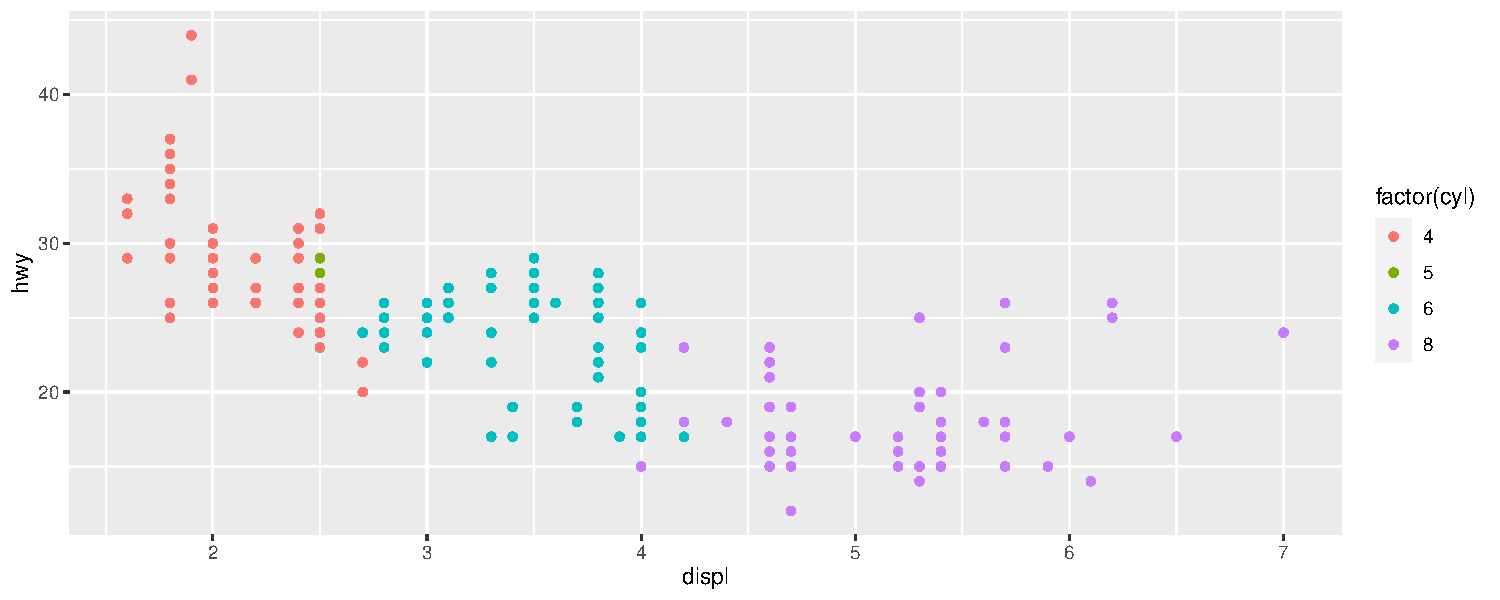
\includegraphics[width=\textwidth]{picture/scatter.pdf}
  \caption{某散点图  \protect\footnotemark} % “\protect\footnotemark”命令是为了在标题中使用脚注的一种曲线救国方法
  \label{fig:scatter}
\end{figure}

\footnotetext{你可能注意到,图片的标题在下方,而表格的标题在下方。这么做的原因可以见 \href{https://tex.stackexchange.com/questions/3243/why-should-a-table-caption-be-placed-above-the-table}
{Stack Exchange}。}
% 注意,若要在图表中的caption使用脚注,就要按这种方式,而不能直接在caption种使用 \footnote 命令
% 详见 https://tex.stackexchange.com/questions/10181/using-footnote-in-a-figures-caption

图~\ref{fig:left} 和图~\ref{fig:right} 是两张并排的图片。图~\ref{fig:photos} 含有4个子图。
\begin{figure}[htbp]
\centering
\begin{minipage}[t]{0.48\textwidth}
\centering
  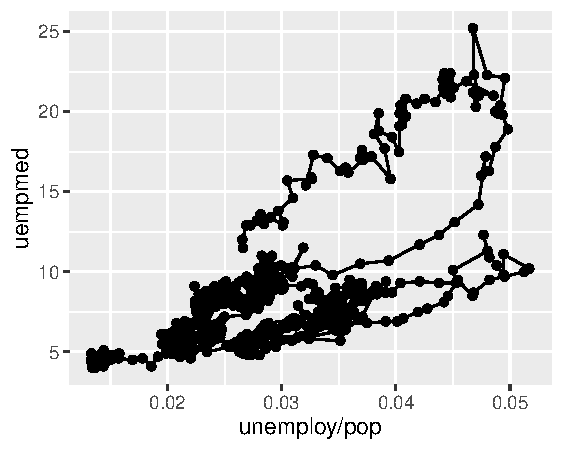
\includegraphics[width=\textwidth]{picture/left.pdf}
  \caption{某路径图}
  \label{fig:left} % 下面要空一格

\end{minipage}
\begin{minipage}[t]{0.48\textwidth}
\centering
  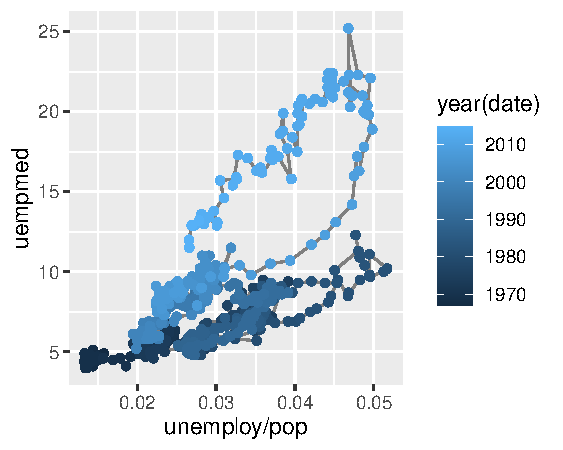
\includegraphics[width=\textwidth]{picture/right.pdf}
  \caption{用颜色区分时间}
  \label{fig:right}
\end{minipage}
\end{figure}

\begin{figure}[htbp]
     \centering
     \begin{subfigure}[b]{.5\linewidth - 1mm}
         \centering
         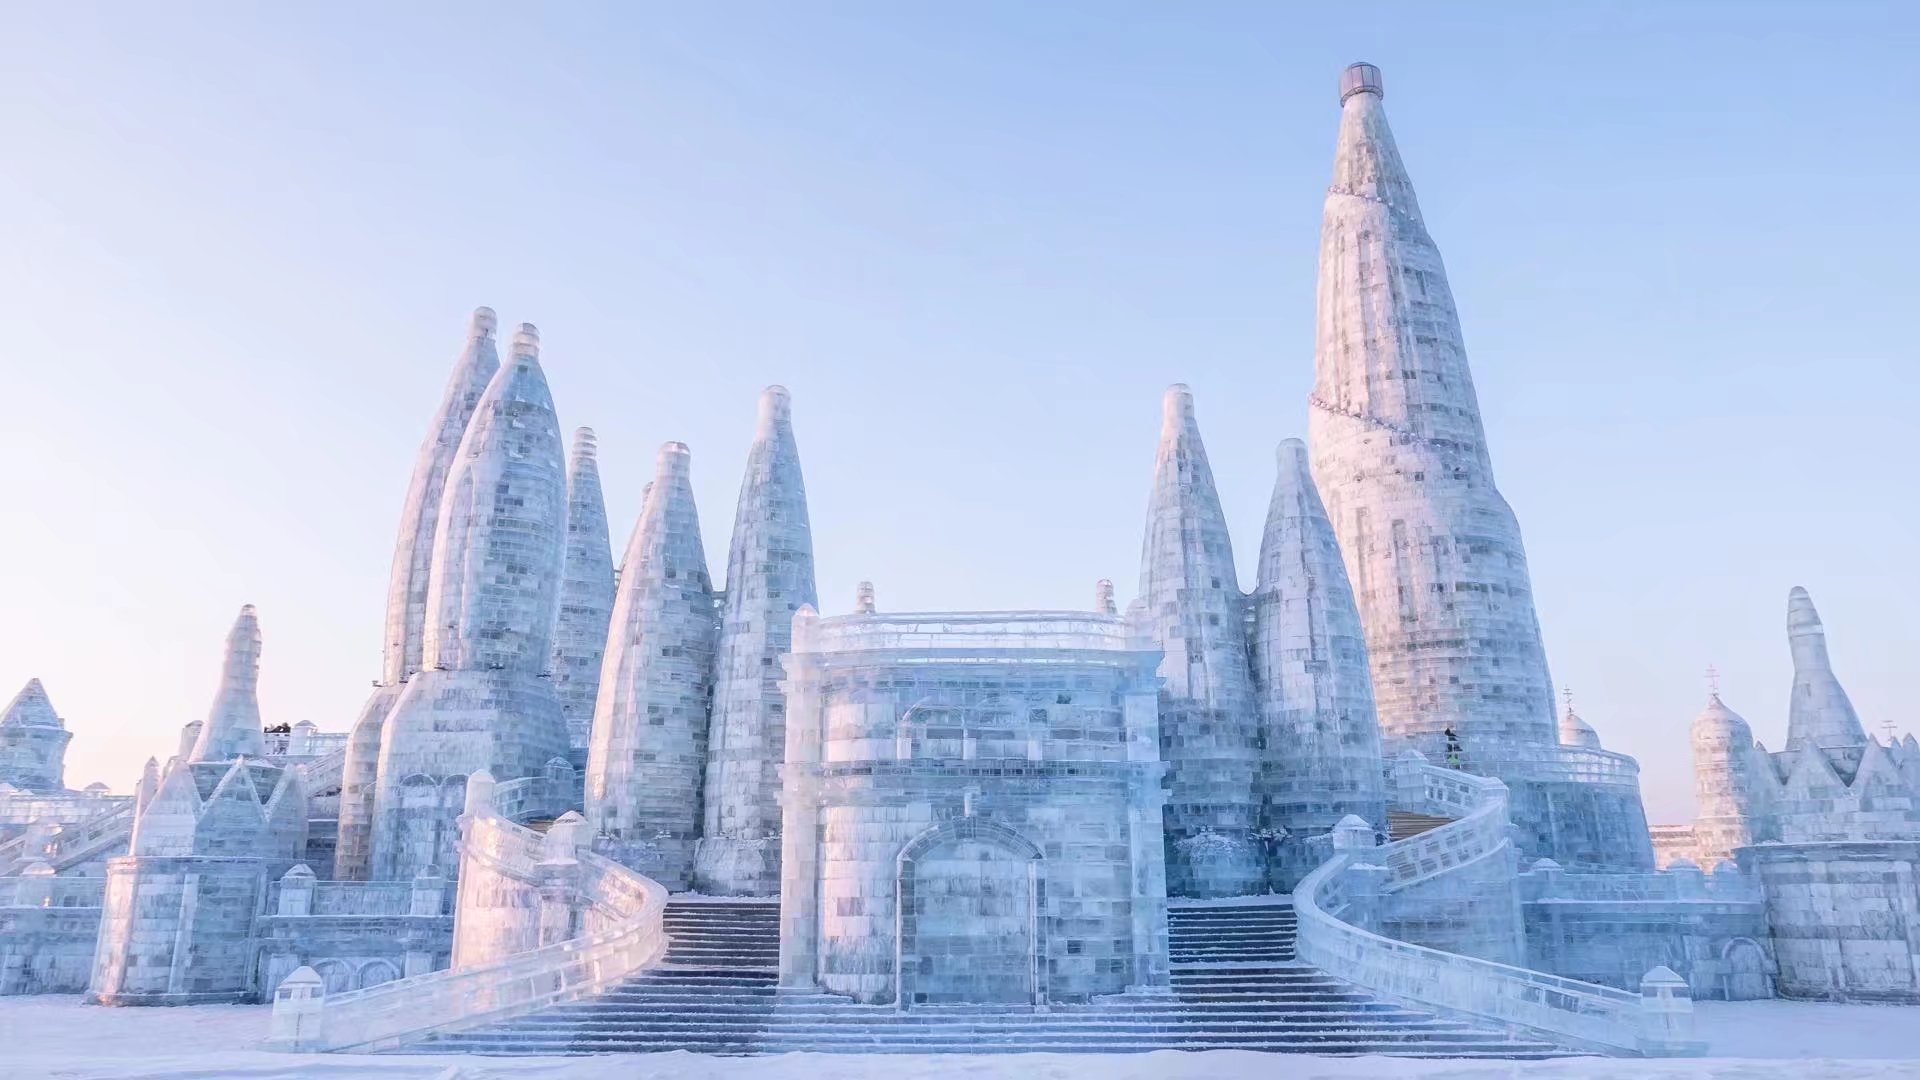
\includegraphics[width=\textwidth]{picture/冰雪大世界.jpg} % 裁剪:,trim=0 12 0 12,clip
         \caption{冰雪大世界}
         \label{fig:冰雪大世界}
     \end{subfigure}
     \hfill
     \begin{subfigure}[b]{.5\linewidth - 1mm}
         \centering
         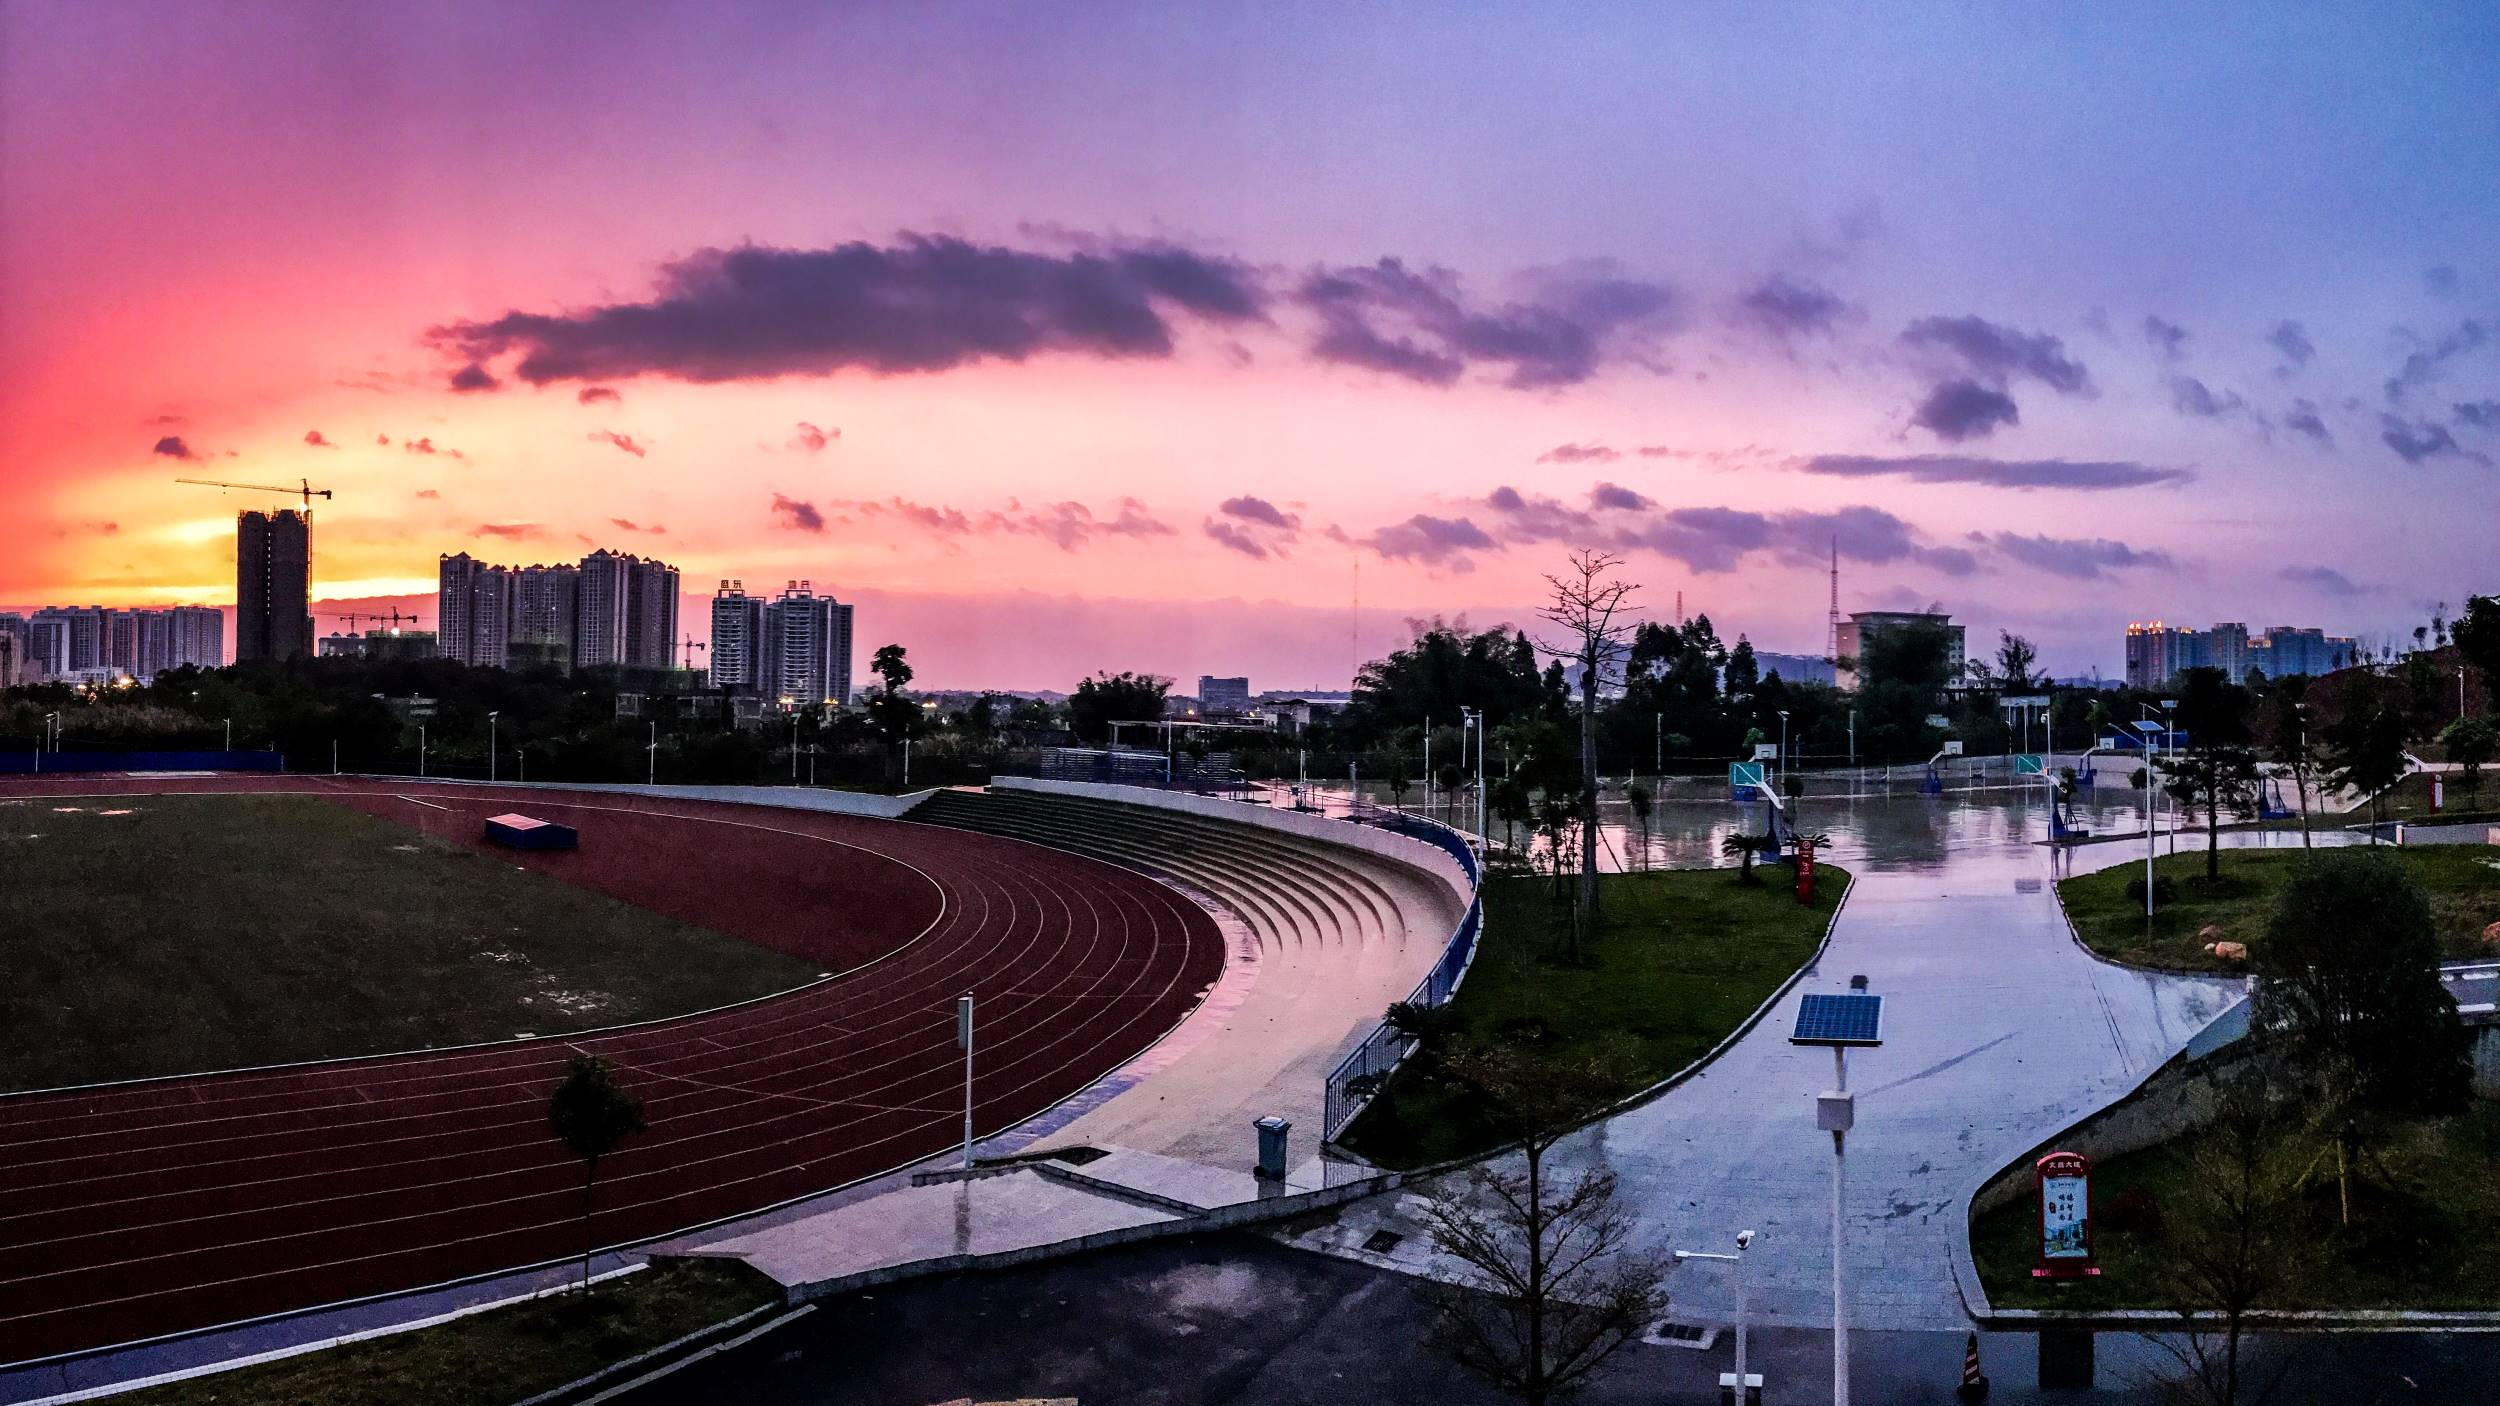
\includegraphics[width=\textwidth]{picture/高中の夕阳.jpg}
         \caption{高中の夕阳}
         \label{fig:高中夕阳}
     \end{subfigure}

     \begin{subfigure}[b]{.5\linewidth - 1mm}
         \centering
         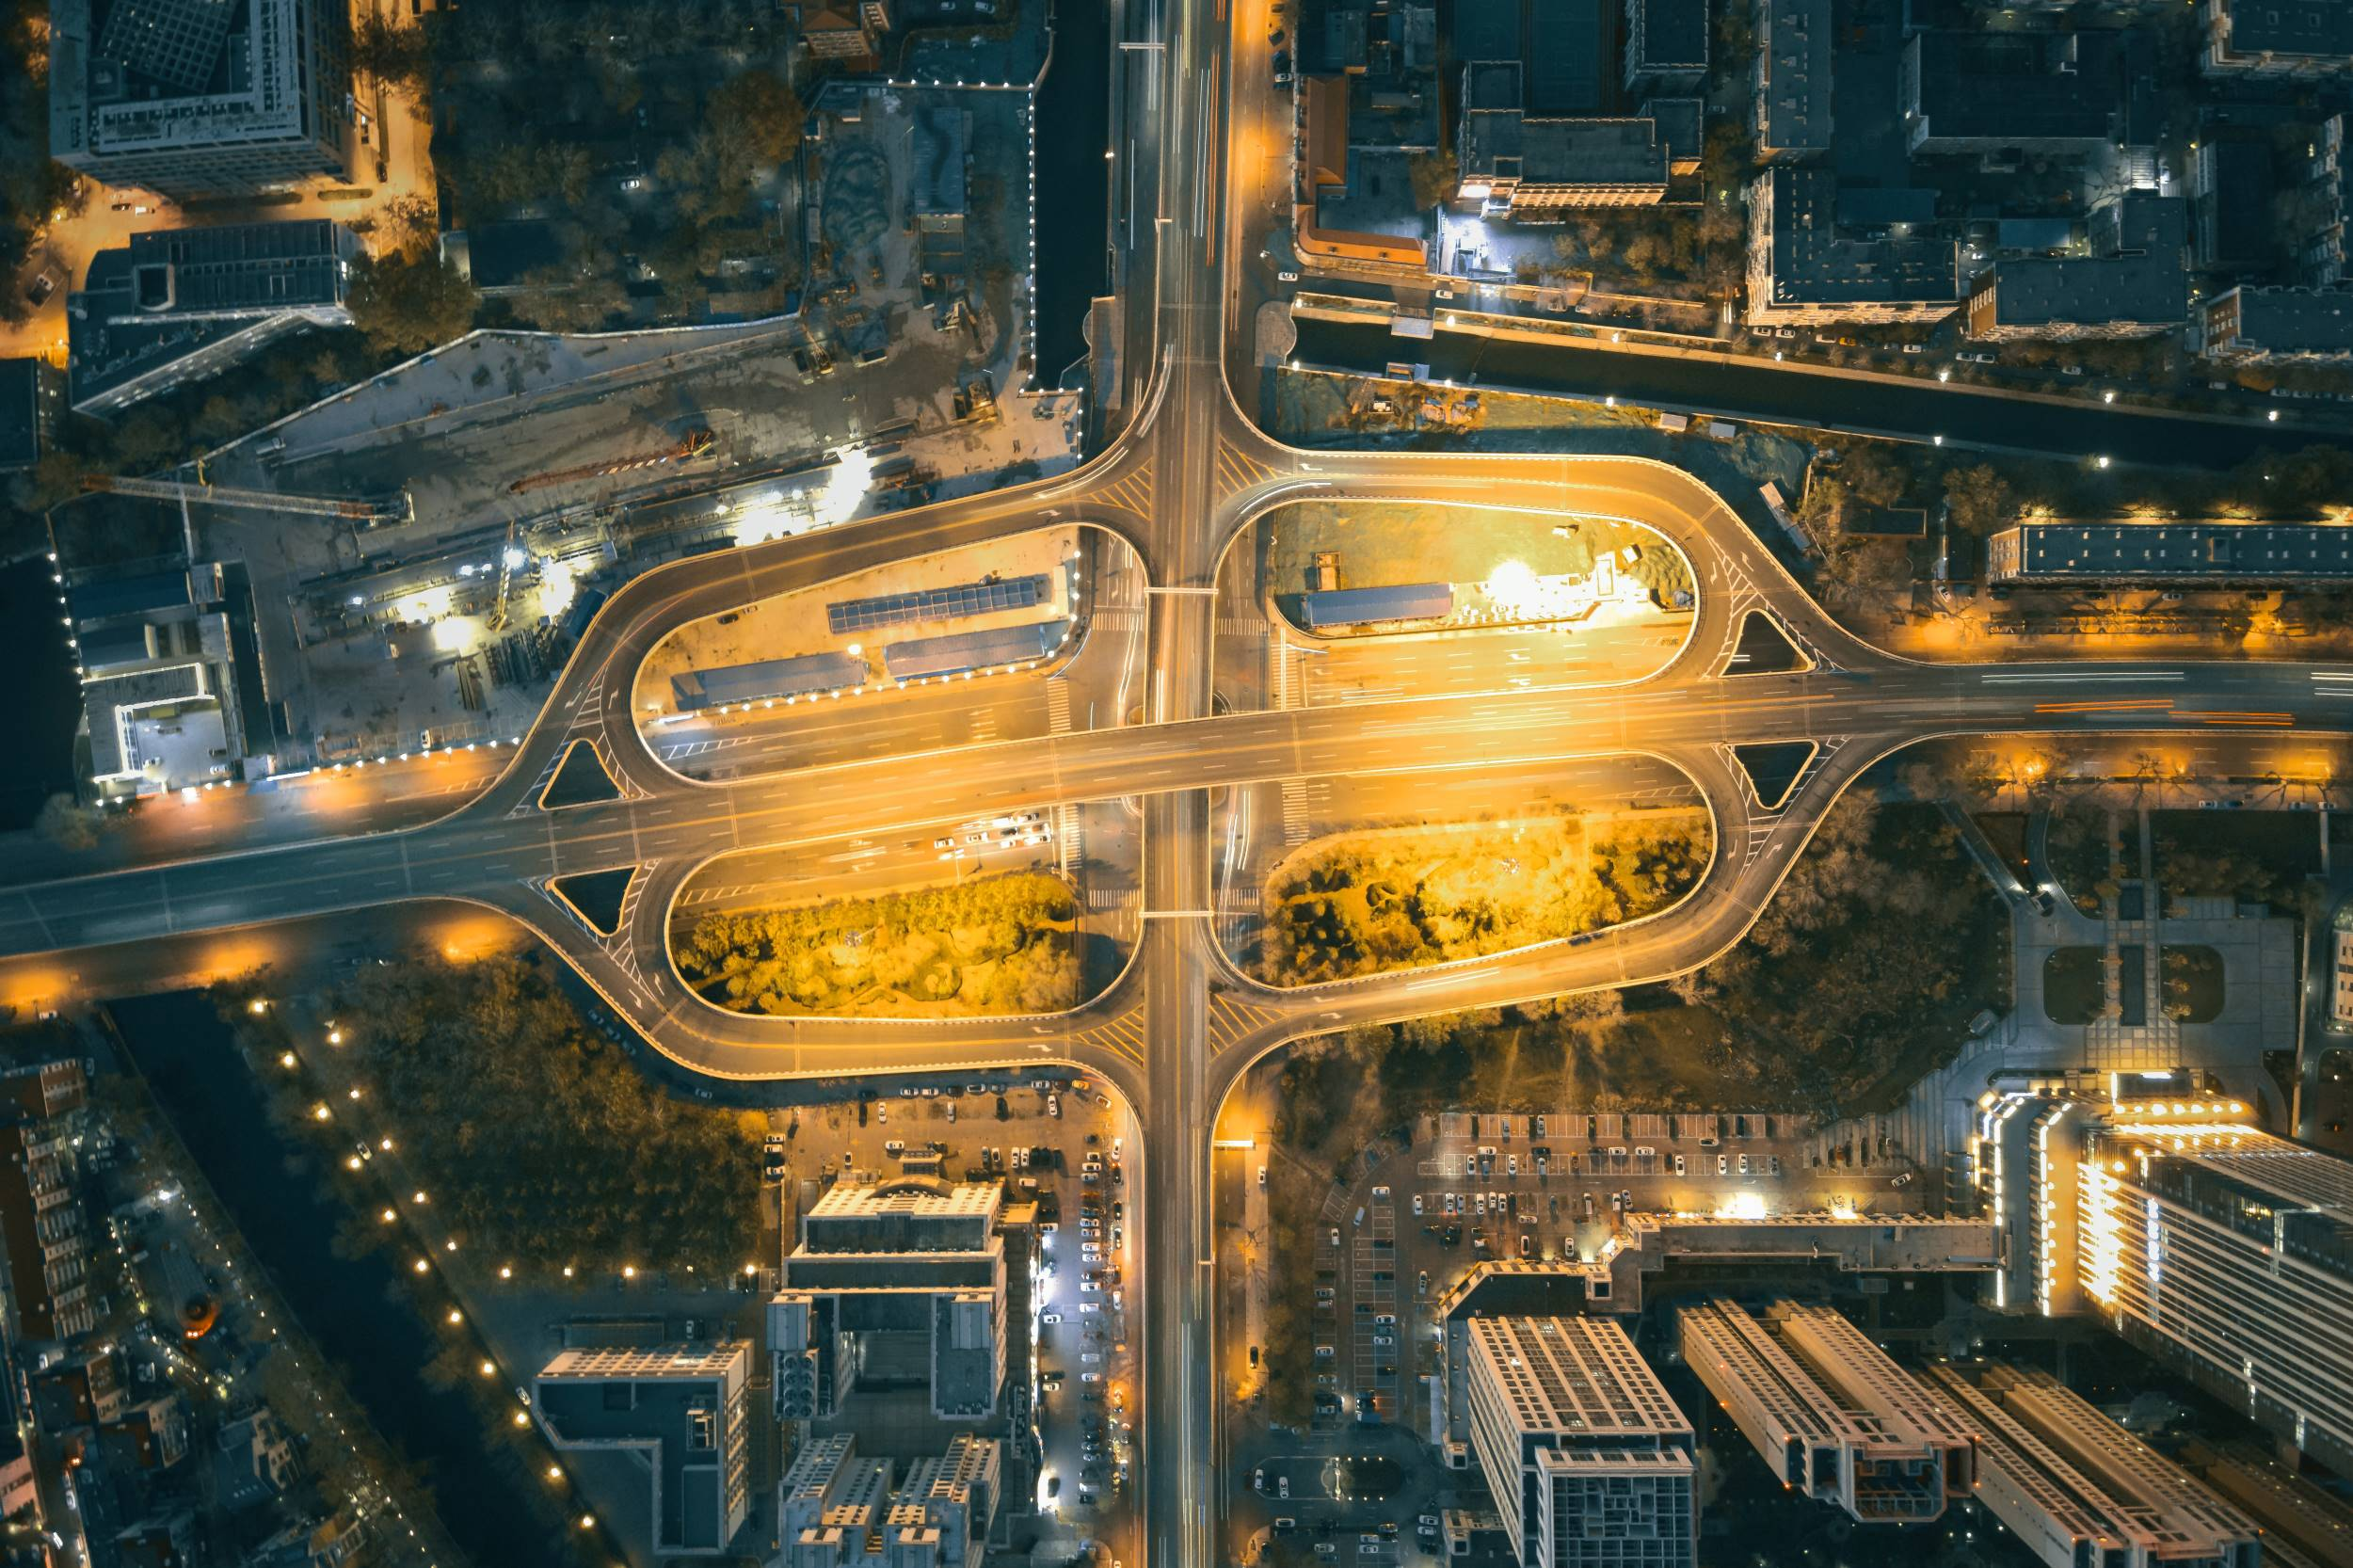
\includegraphics[width=\textwidth]{picture/八里台桥.jpg}
         \caption{八里台桥}
         \label{fig:八里台桥}
     \end{subfigure}
     \hfill
     \begin{subfigure}[b]{.5\linewidth - 1mm}
         \centering
         
\includegraphics[width=\textwidth]{picture/某同学.jpg}
         \caption{作者得不到的同学}
         \label{fig:某同学}
     \end{subfigure}
        \caption{作者拍的照片}
        \label{fig:photos}
\end{figure}



\clearpage
\subsection{表格}
表~\ref{tab:notation1} 用三线表的形式进行符号说明。若完整的表格过长,可以像表~\ref{tab:notationlong} 那样放在附录,在正文仅保留关键的%
符号。
\begin{table}[htbp]
\centering
\caption{符号表示1}
\label{tab:notation1}
\begin{tabular}{@{}cl@{}}
\toprule
\multicolumn{1}{c}{符号} & \multicolumn{1}{c}{描述} \\
\midrule

  $K$ & 产品数 ($k \in\{1,...,K\}$) \\
  $T$ & 周期数 ($t \in\{1,...,T\}$) \\
%  $\delta_k$ & target δ-service level for product k \\
  $c_t$      & $t$时期的产能  \\ % production capacity in period t
%  $c^r_t$    & Remanufacturing capacity in period t  \\
  $hc_k$     & 每周期每单位产品$k$的持有成本   \\ % holding cost of product k per unit and period                                \\
  $q_{kt}$   &  $t$时期产品$k$的产量 \\ % production quantity of product k in period t
  $q^r_{kt}$   &  $t$时期产品$k$的再制造数量 \\ % remanufacturing quantity of product k in period t

\bottomrule
\end{tabular}
\end{table}

表~\ref{tab:ZhangSan1} 也是三线表,但与前者不同,它是二维的,“姓名”和“学科”唯一决定了成绩。将其用表~\ref{tab:ZhangSan2} 展示可以更清晰的看到这一点。

\begin{table}[htbp] % htbp控制浮动,如果你不懂这是什么意思,照抄就OK
  \centering
  \caption{学生的成绩1}\label{tab:ZhangSan1}
  \begin{tabular}{*{6}{c}}
  \bottomrule
  \multirow{2}*{姓名} & \multicolumn{2}{c}{文科} &
      \multicolumn{2}{c}{理科} & \\
  \cmidrule(lr){2-3}\cmidrule(lr){4-5}\cmidrule(lr){6-6}
      \morecmidrules\cmidrule(lr){6-6}
  & 历史 & 文学 & 物理 & 化学 & 总评 \\
  \midrule
  张三 & A & A & B & A & A \\
  李四 & C & B & A & B & B \\
  \bottomrule
  \end{tabular}
\end{table}

\begin{table}[htbp] % htbp控制浮动,如果你不懂这是什么意思,照抄就OK
  \centering
  \caption{学生的成绩2}\label{tab:ZhangSan2}
  \begin{tabular}{|c|*{5}{c}|}
\hline
\diagbox{姓名}{科目} & 历史 & 文学 & 物理 & 化学 & 总评 \\
\hline
  张三 & A & A & B & A & A \\
  李四 & C & B & A & B & B \\
  \hline
  \end{tabular}
\end{table}

\clearpage
\section{数学公式}
\subsection{行内公式}\label{subsec:inlineEqn}
使用\texttt{\$\dots\$}得到行内公式,如$x \in [0, 1]$,$\int_{0}^{\pi} \sin x \, dx = 2$。

\subsection{单行公式}\label{subsec:displayEqn}
使用\texttt{equation}环境得到带编号公式,如式~\eqref{eq:1} 所示。
\begin{equation}\label{eq:1}
  \boldsymbol{\alpha}^2\sum_{j \in \mathbf{N}} b_{ij}
  \hat{y}_{j} = \sum_{j \in \mathbf{N}}
  b^{(\lambda)}_{ij}\hat{y}_{j} + (b_{ii} - \lambda_{i}) \hat{y}_{i} \hat{y}
\end{equation}
而通过\texttt{equation*}得到无编号公式,如
\[
    A = \{ x \in X \mid x \in X_{i}, \text{ 对某些$i \in I$ } \}
\]
无编号公式也可以通过\texttt{\textbackslash [ \dots \textbackslash ]}得到,这是\texttt{equation*}的简写版本。按照要求,所有公式或都编号,或都不编号,虽然作者并没有遵循这一要求。绝大部分数学环境都有带*的版本,它们将不会对公式编号,下文不再赘述。




\subsection{多行公式}\label{subsec:multiEqn}
使用\texttt{align}\footnote{\texttt{align}环境还可以对多列进行对齐,此处只展示了对一列对齐。}环境可以指定公式在某处对齐,这里我们使公式沿等号左侧对齐(在代码中用\&表示对齐点):
\begin{align}\label{eq:align}
  x &= y \times z  \\
  dz &= x + y
\end{align}
若想用下一级编号,可以用\texttt{subequation}环境包围\texttt{align},或其他多公式环境\footnote{有关微分算子应该用直立体还是斜体,可以见 \href{https://tex.stackexchange.com/questions/14821/whats-the-proper-way-to-typeset-a-differential-operator}{Stack Exchange} 的讨论。}:
\begin{subequations}\label{eq:subEqn}
  \begin{align}
  x &= y \times z  \\
  \mathrm{d}z &= x + y
\end{align}
\end{subequations}

\texttt{alignat}环境与\texttt{align}环境类似,区别在于前者需要手动设置列之间的间距,而后者会对其自动设置。
我们可以用\texttt{alignat}排版带有注释的公式:
\begin{alignat}{2}
    x &= x \wedge (y \vee z) &
    &\quad\text{(by distributivity)}\\
        &= (x \wedge y) \vee (x \wedge z) & &
            \quad\text{(by condition (M))}\notag\\
        &= y \vee z \notag
\end{alignat}
或方程组:
\begin{subequations}
\begin{alignat}{4}
a_{11}x_1 &+ a_{12}x_2 &&+ a_{13}x_3  &&                   &&= y_1,\\
a_{21}x_1 &+ a_{22}x_2 &&                    &&+ a_{24}x_4 &&= y_2,\\
a_{31}x_1 &                   &&+ a_{33}x_3  &&+ a_{34}x_4 &&= y_3.
\end{alignat}
\end{subequations}


有时候我们不想指定公式具体沿哪里对齐,而只是想将它们居中放置,使用\texttt{gather}环境可以达到这个目的。
\begin{gather}
    3(a-x) = 3.5x + a - 1 \\
    a = \frac{13}{4}x - \frac{1}{2} \\
\end{gather}

使用 \texttt{\textbackslash intertext}可以在公式中插入一行文字,如:
\begin{subequations}
    \begin{align}
        h(x) &= \int \left(\frac{ f(x) + g(x) } {1 + f^{2}(x)} + \frac{1 + f(x)g(x)} { \sqrt{1 - \sin x} } \right) \, dx \label{eq:textUp} \\
        \intertext{化简为}
        &= \int \frac{1 + f(x)} {1 + g(x)} \, dx - 2 \arctan(x - 2) \ \label{eq:textLow}
    \end{align}
\end{subequations}
注意到虽然中间有一行字,但式~\eqref{eq:textUp} 和式~\eqref{eq:textLow} 仍在同一个数学公式中。


\subsection{多行的单公式}
本小节提及的环境,都需要嵌套于前面的小节提及的数学环境中。例如,若想使用\texttt{aligned}环境(\texttt{align}的行内版本),需要将其放于\texttt{equation}等数学环境中。整个\texttt{aligned}环境作为一个整体,成为父环境的一个元素。

我们使用\texttt{aligned}将不同的行沿等号左侧对齐:
\begin{equation}\label{eq:aligned}
  \begin{aligned}
    \arctan'(x) &=(h^{-1})'(x) \\
                     &= \frac{1}{h'(h^{-1}(x))} \\
                     &= \frac{1}{\tan '(\arctan x)} \\
                     &= \frac{1}{\sec^{2}(\arctan x)}
  \end{aligned}
\end{equation}
注意到它只会对整个公式居中编号,而不像式~\eqref{eq:align} 对每行都进行编号。
更复杂的例子如下,我们令他们沿最左侧对齐,并且在后3行的行首加入了长度不等的空白。
\begin{equation*}
  \begin{aligned}
    &\bar{J}^{i}\left(\alpha_{t}^{i, \star};\boldsymbol{\mu}\right)-\bar{J}^{i}\left(\hat{\alpha}_{t}^{i, \star} ; \hat{\boldsymbol{\mu}}\right)+\lambda^{k} \mathbb{E}\left[\int_{0}^{T}\left\|\alpha_{t}^{i, \star}-\hat{\alpha}_{t}^{i, \star}\right\|^{2} d t\right]
    \\
    &\quad\leq\mathbb{E}\left[\int_{0}^{T}\left(\dfrac{\zeta^{k}}{2}\left(\hat{g}_{t}^{i, \star}-h_{t}^{k}\right)^{2}+\dfrac{\gamma^{k}}{2}\left(\hat{\Gamma}_{t}^{i, \star}\right)^{2}+S_{t}^{\mu} \hat{\Gamma}_{t}^{i, \star}\right) d t+P F_{\delta}^{\prime}\left(R^{k}-\hat{X}_{T}^{i}\right)\right]
    \\
    &\qquad -\mathbb{E}\left[\int_{0}^{T}\left(\dfrac{\zeta^{k}}{2}\left(\hat{g}_{t}^{i, \star}-h_{t}^{k}\right)^{2}+\dfrac{\gamma^{k}}{2}\left(\hat{\Gamma}_{t}^{i, \star}\right)^{2}+S_{t}^{\hat{\mu}} \hat{\Gamma}_{t}^{i, \star}\right) d t+P F_{\delta}^{\prime}\left(R^{k}-\hat{X}_{T}^{i}\right)\right]
     \\
    &\quad =\mathbb{E}\left[\int_{0}^{T} \hat{\Gamma}_{t}^{i, \star}\left(S_{t}^{\mu}-S_{t}^{\hat{\mu}}\right) d t\right].
  \end{aligned}
\end{equation*}

下面这种if-else情况可以用\texttt{cases}环境生成:
\begin{equation}
  f(x)
    = \begin{cases}
    -x^{2},            &\text{$x < 0$;}\\
    \alpha + x,     &\text{$0 \leq x \leq 1$;}\\
    x^{2},             &\text{其它.}
    \end{cases}
\end{equation}


目前为止我们都是单独地使用多行的单公式。实际上我们也可以将其放入多行公式中: % 只能用split,内外的 & 可以对齐
\begin{align} % split 的& 可以被外层的 align识别。若用aligned替换align,则无法达到该效果
\begin{split}
f &= (x_{1} x_{2} x_{3} x_{4} x_{5} x_{6})^{2}\\
&= (x_{1} x_{2} x_{3} x_{4} x_{5} + x_{1} x_{3} x_{4} x_{5} x_{6} + x_{1} x_{2} x_{4} x_{5} x_{6} + x_{1} x_{2} x_{3} x_{5} x_{6})^{2}, \end{split}\\
g &= y_{1} y_{2} y_{3}.
\end{align}
这里我们在多行公式中使用了多行的单公式。可以看到,前两行是一个公式,最后一行是另一个公式。

下面展示了一些矩阵,它们本身是多行的,作为整体被视为父公式的一个部分。
\[
\begin{pmatrix}
1 & 2 & 3\\
a & b & c
\end{pmatrix}
\quad
\begin{bmatrix}
1 & 2 & 3\\
a & b & c
\end{bmatrix}
\quad
\begin{vmatrix}
1 & 2 & 3\\
a & b & c
\end{vmatrix}
\quad
\begin{bmatrix}
1 & 0 & \cdots & 0 \\
 0 & 1 & \cdots & 0 \\
 \vdots & \vdots & \ddots & \vdots \\
 0 & 0 & \cdots & 1
 \end{bmatrix}
\]

\section{类定理环境示例}
\begin{definition}[上确界与下确界]\label{def:supremum}
\leavevmode % 如果不需要从下一行开始,则可以删去此行
\begin{enumerate}[label=(\arabic*),leftmargin=2\parindent]
  \item 如果数集$S$的上界集中有最小值,则称之为$S$的\textbf{上确界},记为$\sup S$;
  \item 如果数集$S$的下界集中有最大值,则称之为$S$的\textbf{下确界},记为$\inf S$。
\end{enumerate}
\end{definition}

% 注意 \ref 两边的空格,会导致数字与两侧的汉字留有一定间距,更加美观
从定义~\ref{def:supremum} 容易看到,如果数集$S$有上(下)确界,则它的上(下)确界是唯一的。以上定义中sup是supermum的简写,而inf是infimum的简写。设$\beta = \sup S$,这包含两层意思:\begin{enumerate*}[label=(\roman*)]
\item $\beta$是$S$的上界,即对任意$x \in S$,都成立$x\leqslant \beta$;
\item $\beta$是$S$的所有上界中最小的,即对任意$\varepsilon > 0$,$\beta - \varepsilon$都不是$S$的上界,亦即对任意$\varepsilon > 0$,都存在$x_0 \in S$,使得$x_0 > \beta - \varepsilon$。
\end{enumerate*}
总结如下:
\begin{theorem}\label{thm:1}
$\beta$是数集$S$的上确界的充分必要条件是
\begin{enumerate}[label=\textup{(\arabic*)},leftmargin=2\parindent]
  \item 对任意$x \in S$,都成立$x \leq \beta$;
  \item 对任意$\varepsilon > 0$,都存在$x_0 \in S$,使得$x_0 > \beta - \varepsilon$。
\end{enumerate}
\end{theorem}
对于下确界也有类似的定理。


\begin{corollary}[确界原理]\label{cor:1}
有下界的非空数集必有下确界。
\end{corollary}

\begin{proof}
  设$S$是一个有下界的非空数集。于是$T = \{-x \mid x \in S\}$非空有上界,因而有上确界,设$\beta = \sup T$。记$\alpha = -\beta$,于是$\alpha = \inf S$。
\end{proof}

\begin{remark}
我也不知道有什么好注的,告诉你可以这么用而已。
\end{remark}

\begin{theorem}[单调收敛定理]\label{thm:monotone}
  单调有界数列必收敛,具体地说:
  \begin{enumerate}[label=\textup{(\arabic*)}]
    \item 若数列$\{x_n \}$递增且有上界,则
    \[\lim_{n \to \infty} x_n = \sup\{x_n \mid n \in \mathbb{N} \}; \]

    \item 若数列$\{x_n \}$递减且有下界,则
    \[\lim_{n \to \infty} x_n = \inf \{x_n \mid n \in \mathbb{N} \}. \]
  \end{enumerate}
\end{theorem}

\begin{lemma}\label{lem:1}
Let $a < b < c$ and let $f$ be continuous on the interval $[a, c]$. Let $\varepsilon > 0$, and suppose that statements hold.
Then there is a $\delta > 0$ such that, if $x$ and $y$ are in $[a, c]$ and $\left|x - y\right| < \delta$, then $\left|f(x) - f(y)\right| < \varepsilon$.
\end{lemma}

\begin{assumption}\label{assum:1}
The proportion of the total population of agents belonging to each class
$k$ converges to a constant as the number of firms ($N$) increases.
\end{assumption}


\section{数字和单位}
表~\ref{tab:number} 展示了一些数字和单位的写法,以及常见的错误写法。
\begin{table}[htbp]
\centering
\caption{数字与单位示范}\label{tab:number}
\begin{tabular}{@{}ll@{}}
\toprule
\multicolumn{1}{c}{优秀范例} & \multicolumn{1}{c}{没那么好} \\ \midrule
\num{12345,67890} & 12345.67890 \\
\num{1+-2i} & 1 $\pm$ 2i \\
\num{.3e45} & 0.3 $\times$ 10\textsuperscript{45} \\
\num{1.654 x 2.34 x 3.430} & 1.654 x 2.34 x 3.430 \\
\si{\kilo\gram\metre\per\square\second} & kg m s\textsuperscript{-2} \\
\si{\square\volt\cubic\lumen\per\farad} & $V^{2}lm^{3}F^{-1}$ \\
\SI[mode=text]{1.23}{J.mol^{-1}.K^{-1}} & 1.23J mol\textsuperscript{-1}K\textsuperscript{-1} \\
%\SI{.23e7}{\candela} & 0.23 $\times$ 10\textsuperscript{7}cd \\
\SI[per-mode=symbol]{1.99}[\$]{\per\kilogram} & \$ 1.99/kg \\
\SI[per-mode=fraction]{1,345}{\coulomb\per\mole} & 1.345$\frac{C}{mol}$ \\ \bottomrule
\end{tabular}
\end{table}


\section{代码与算法}
我们可以使用 \href{https://ctan.org/pkg/listings?lang=en}{\texttt{listings}} 排版代码。它支持多种语言,如C, C++, JAVA, Matlab, R, Python等,完整语言支持见\href{https://ctan.mirrors.hoobly.com/macros/latex/contrib/listings/listings.pdf}{文档}的2.4节(Programming languages)。
代码~\ref{code:fibonacci} 用Python实现了通过递推的方式计算斐波那契数列,以防止栈溢出。
% 使用caption会生成标题,而用title则不会
\begin{lstlisting}[language=Python, caption=计算斐波那契数列,label=code:fibonacci]
def fibonacci(n):
    if n == 1:
        return 1
    elif n == 2:
        return 2
    else:
        curr, prev, i = 3, 2, 3     # 从 fib 3 开始计算
        while i != n:
            i, curr, prev = i+1, curr+prev, curr

        return curr
\end{lstlisting}
% \lstinputlisting[language=Python, caption=代码示例:计算斐波那契数列(Python),label=code:fibonacci]{fibonacci.py}
% 你也可以像这样引用本地文件,而不是直接将代码写在tex文件中

我们可以使用 \href{https://ctan.org/pkg/algorithms}{\texttt{algorithms}} 包排版算法。算法~\ref{algo:1} 将指数计算的复杂度由$O(n)$降到了$O(\log n)$。
\begin{algorithm}
  \caption{加速指数计算}
  \label{algo:1}
  \begin{algorithmic}
  \REQUIRE $n \geq 0 \vee x \neq 0$
  \ENSURE $y = x^n$
  \STATE $y \gets 1$
  \IF{$n < 0$}
  \STATE $X \gets 1 / x$
  \STATE $N \gets -n$
  \ELSE
  \STATE $X \gets x$
  \STATE $N \gets n$
  \ENDIF
  \WHILE{$N \neq 0$}
  \IF{$N$ is even}
  \STATE $X \gets X \times X$
  \STATE $N \gets N / 2$
  \ELSE[$N$ is odd]
  \STATE $y \gets y \times X$
  \STATE $N \gets N - 1$
  \ENDIF
  \ENDWHILE
  \end{algorithmic}
\end{algorithm}


%\section{化学方程式}
%由于个人觉得化学专业一般不太用\LaTeX,因此仅作少量演示。
%
%可以使用 \href{https://ctan.org/pkg/mhchem?lang=en}{\texttt{mhchem}} 宏包制作化学方程式,如:
%\begin{center}
%    \ce{Na2SO4 ->[H2O] Na+ + SO4^2-} \\
%    \ce{(2Na+,SO4^2- ) + (Ba^2+, 2Cl- ) -> BaSO4 v + 2NaCl}
%\end{center}



\NKUAppendixSection % 附录节
附录内容一般包括正文中不便列出的冗长公式推导、符号说明(含缩写)、计算机程序等。
(不过按照毕业论文指导手册的意思,只能有一个附录吗。)

\begin{center}
\begin{longtable}{|l|l|l|}
\caption{宜放在附录的长表格} \label{tab:long} \\

\hline \multicolumn{1}{|c|}{\textbf{First column}} & \multicolumn{1}{c|}{\textbf{Second column}} & \multicolumn{1}{c|}{\textbf{Third column}} \\ \hline
\endfirsthead

\multicolumn{3}{c}%
{{ \ 续表~\thetable{}}} \\
\hline \multicolumn{1}{|c|}{\textbf{First column}} & \multicolumn{1}{c|}{\textbf{Second column}} & \multicolumn{1}{c|}{\textbf{Third column}} \\ \hline
\endhead

\hline \multicolumn{3}{|r|}{{接下页}} \\ \hline
\endfoot

\hline \hline
\endlastfoot

One & abcdef ghjijklmn & 123.456778 \\
One & abcdef ghjijklmn & 123.456778 \\
One & abcdef ghjijklmn & 123.456778 \\
One & abcdef ghjijklmn & 123.456778 \\
One & abcdef ghjijklmn & 123.456778 \\
One & abcdef ghjijklmn & 123.456778 \\
One & abcdef ghjijklmn & 123.456778 \\
One & abcdef ghjijklmn & 123.456778 \\
One & abcdef ghjijklmn & 123.456778 \\
One & abcdef ghjijklmn & 123.456778 \\
One & abcdef ghjijklmn & 123.456778 \\
One & abcdef ghjijklmn & 123.456778 \\
One & abcdef ghjijklmn & 123.456778 \\
One & abcdef ghjijklmn & 123.456778 \\
One & abcdef ghjijklmn & 123.456778 \\
One & abcdef ghjijklmn & 123.456778 \\
One & abcdef ghjijklmn & 123.456778 \\
One & abcdef ghjijklmn & 123.456778 \\
One & abcdef ghjijklmn & 123.456778 \\
One & abcdef ghjijklmn & 123.456778 \\
One & abcdef ghjijklmn & 123.456778 \\
One & abcdef ghjijklmn & 123.456778 \\
One & abcdef ghjijklmn & 123.456778 \\
One & abcdef ghjijklmn & 123.456778 \\
One & abcdef ghjijklmn & 123.456778 \\
One & abcdef ghjijklmn & 123.456778 \\
One & abcdef ghjijklmn & 123.456778 \\
One & abcdef ghjijklmn & 123.456778 \\
One & abcdef ghjijklmn & 123.456778 \\
One & abcdef ghjijklmn & 123.456778 \\
One & abcdef ghjijklmn & 123.456778 \\
One & abcdef ghjijklmn & 123.456778 \\
One & abcdef ghjijklmn & 123.456778 \\
One & abcdef ghjijklmn & 123.456778 \\
One & abcdef ghjijklmn & 123.456778 \\
One & abcdef ghjijklmn & 123.456778 \\
One & abcdef ghjijklmn & 123.456778 \\
One & abcdef ghjijklmn & 123.456778 \\
One & abcdef ghjijklmn & 123.456778 \\
One & abcdef ghjijklmn & 123.456778 \\
One & abcdef ghjijklmn & 123.456778 \\
One & abcdef ghjijklmn & 123.456778 \\
One & abcdef ghjijklmn & 123.456778 \\
One & abcdef ghjijklmn & 123.456778 \\
One & abcdef ghjijklmn & 123.456778 \\
One & abcdef ghjijklmn & 123.456778 \\
One & abcdef ghjijklmn & 123.456778 \\
One & abcdef ghjijklmn & 123.456778 \\
One & abcdef ghjijklmn & 123.456778 \\
One & abcdef ghjijklmn & 123.456778 \\
One & abcdef ghjijklmn & 123.456778 \\
One & abcdef ghjijklmn & 123.456778 \\
One & abcdef ghjijklmn & 123.456778 \\
One & abcdef ghjijklmn & 123.456778 \\
One & abcdef ghjijklmn & 123.456778 \\
One & abcdef ghjijklmn & 123.456778 \\
One & abcdef ghjijklmn & 123.456778 \\
One & abcdef ghjijklmn & 123.456778 \\
One & abcdef ghjijklmn & 123.456778 \\
One & abcdef ghjijklmn & 123.456778 \\
One & abcdef ghjijklmn & 123.456778 \\
\end{longtable}
\end{center}

表~\ref{tab:notationlong} 展示了较长的符号说明,并将类似的符号归类。为了指定表格的宽度,我们使用了 \texttt{tabularx} 环境,而不是普通的 \texttt{table} 环境
\begin{table}[htbp]
    \caption{较长的符号说明表格}\label{tab:notationlong}
    \begin{tabularx}{\textwidth}{p{0.2\textwidth}X}
    \toprule
      \CJKunderline{索引}\\
      $K$ & number of products ($k \in\{1,...,K\}$)  \\
      $T$ & number of periods ($t \in\{1,...,T\}$)\\

      \CJKunderline{参数} \\
      $\delta_k$ & target $\delta$-service level for product $k$ \\
      $c_t$      & production capacity in period $t$ \\
      $c^r_t$    & remanufacturing capacity in period $t$  \\
      $hc_k$    & holding cost of product $k$ per unit and period   \\
      $hc_k$     & holding cost of product $k$ per unit and period   \\
      $oc$   & overtime costs per unit   \\
      $M_{kt}$   & bignumber for product $k$ in period $t$\\
      $pc_{k}$   & production cost of product $k$ per unit\\
      $pc^r_{k}$ & remanufacturing cost of product $k$ per unit\\
      $sc_{k}$   &  setup cost of product $k$\\
      \CJKunderline{随机变量} \\
      $BL_{kt}$  & backlog of product $k$ at the end of period $t$\\
      $D_{kt}$   & external demand of product $k$ in period $t$  \\
      $I_{kt}$   & net inventory of product $k$ at the end of period $t$  \\
      $I^r_{kt}$ & net inventory of returns of product $k$ at the end of period $t$  \\
      $IP_{kt}$   & physical inventory of product $k$ at the end of period $t$\\
      $IP^r_{kt}$   & physical inventory of recoverables at the end of period $t$\\
      $R_{kt}$   &  returns of product $k$ in period $t$\\
      $SF^r_{kt}$   &  shortfall of recoverables of product $k$ in period $t$\\
      \CJKunderline{决策变量}\\
      $q_{kt}$   &  production quantity of product $k$ in period $t$\\
      $q^r_{kt}$   &  remanufacturing quantity of product $k$ in period $t$  \\
      $o_{t}$   &  amount of overtime for production in period $t$  \\
      $o^r_{t}$   &  amount of overtime for remanufacturing in period $t$\\
      \bottomrule
     \end{tabularx}
    \end{table}


\clearpage
\setcounter{secnumdepth}{0} % 抑制section的编号

\begin{thebibliography}{99}\label{sec:bib}
\addtolength{\itemsep}{-1.5ex} % 缩小行间距,可选
\bibitem{PangQingShan}庞青山.论大学学科组织及其特色.高等理科教育,2005,63(5):1\~{}3.
\bibitem{KohYW}Koh Y W, Lai C S, Loh K, \emph{et al}. Growth of bismuth sulfide mamowire using bismuth trisxanthate single sourceprecursors. Chem Mater, 2003, 15(24): 4544\~{}4554.
\bibitem{LiMing}李明.物理学.北京:科学出版社,1977,58\~{}62.
\bibitem{Dupont}Dupont B. Bone marrow transplantation in severe combined immunodeficiency with an unrelated MLC compatible donor. In:White H J, Smith R, eds. Proceedings of the Third Annual Meeting of the International Society for Experimental Hematology. Houston:International Society for Experimental Hematology, 1974.44\~{}46.
\bibitem{HuGang}胡  刚.蛋白质深度分析以及基因的进化模型:[博士学位论文].天津:南开大学,2005.
\bibitem{YaoGuangQi}姚光起.一种氧气镐材料的制备方法.中国专利.ZL891056088,1980-07-03.
\bibitem{GB3100}中华人民共和国国家技术监督局.GB3100--3102.中华人民共和国国家标准.北京:中国标准出版社,1994-11-01.
\bibitem{url}SREC Trade, New jersey srec market, 2019, \url{https://www.srectrade.com/srec markets/new jersey} (accessed 2019-02-13)\footnote{除本条外,所列的参考文献均来源于\href{http://jwc.nankai.edu.cn/bylwwsjw/list.htm}{《指导手册》}。本条意在演示使用url。}.
\end{thebibliography}



\NKUThanksSection
感谢使用本模板。

Thanks for using this template.

\end{document} 
